%!TEX root = ../dokumentation.tex

\chapter{Introduction}\label{cha:Introduction}
??
matlab version
ascet version
\chapter{D1: Time estimate based on three point estimation}\label{cha:D1}
\begin{table}[H]
\centering
\caption{Three point estimation of effort for meeting requirements}
\begin{adjustbox}{width=1\textwidth, center=\textwidth}
\renewcommand{\arraystretch}{1}
\begin{tabular}{lllllll}
\textbf{Requirement} \textbf{Optimistic} & \textbf{Likely} & \textbf{Pessimistic} & \textbf{<T>} & \textbf{sigmahoch2} & \textbf{Actual}\\\hline
D1 & .& .& .& .& .&\\
\end{tabular}

\end{adjustbox}
\label{tbl:ConceptTPTPProductionSymbols}
\end{table}
\chapter{D2: Feasibility study}\label{cha:D2}
The aim of the feasibility study is to analyse whether the introduced model in section \ref{cha:Introduction} can be implemented based on the given formulas. 

\begin{equation}
	\frac{\partial v}{\partial t} = -c-b*p
\end{equation}
\begin{equation}
	\frac{\partial x}{\partial t} = v
\end{equation}

- Minimale Geschwindigkeit 0,29km/h beachten -> in m/s umrechnen \\
- Switch -> wenn Geschwindigkeit kleiner 0,29 folgt daraus Geschwindigkeit = 0 \\
- Screenshot Simulink Modell und Ergebnis\\
- R5 auch beachtet \\

\begin{figure}[H]
\centering
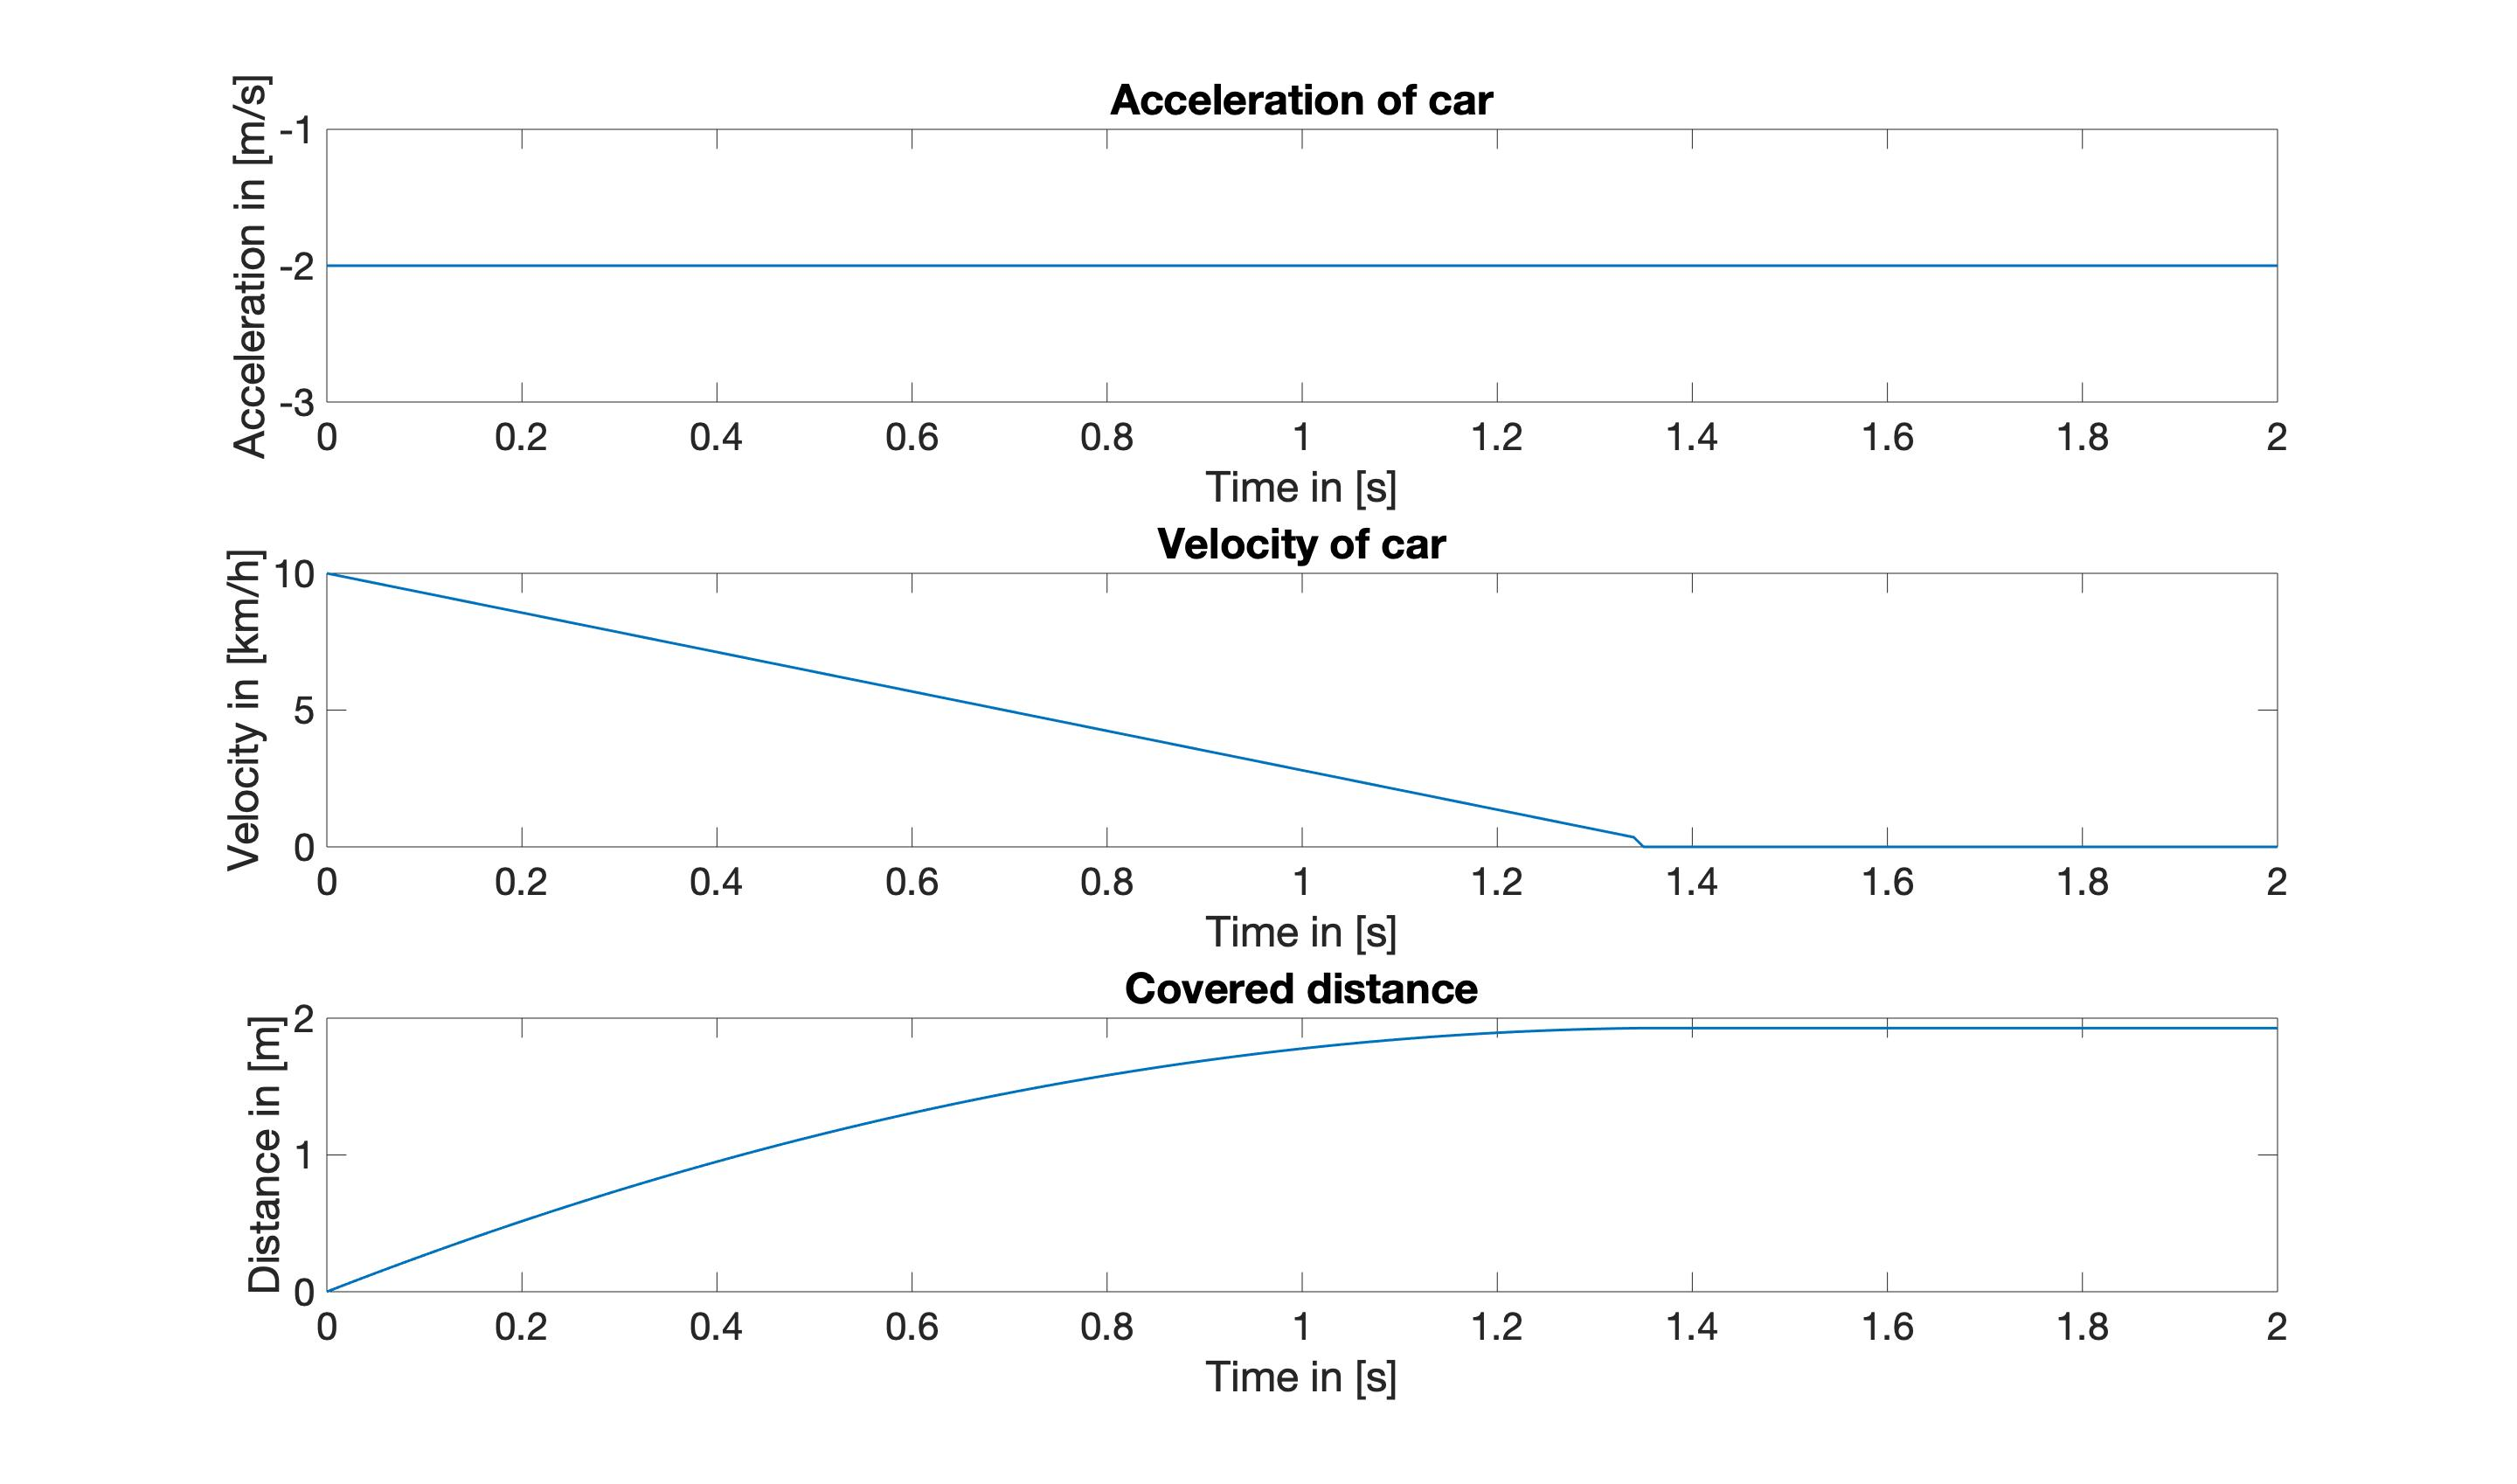
\includegraphics[width=1\textwidth]{images/D2_plot.jpg}
\caption{UML diagram of the architecture of the software tool}
\label{fig:ConceptArchitectureOverview}
\end{figure}

\begin{figure}[H]
\centering
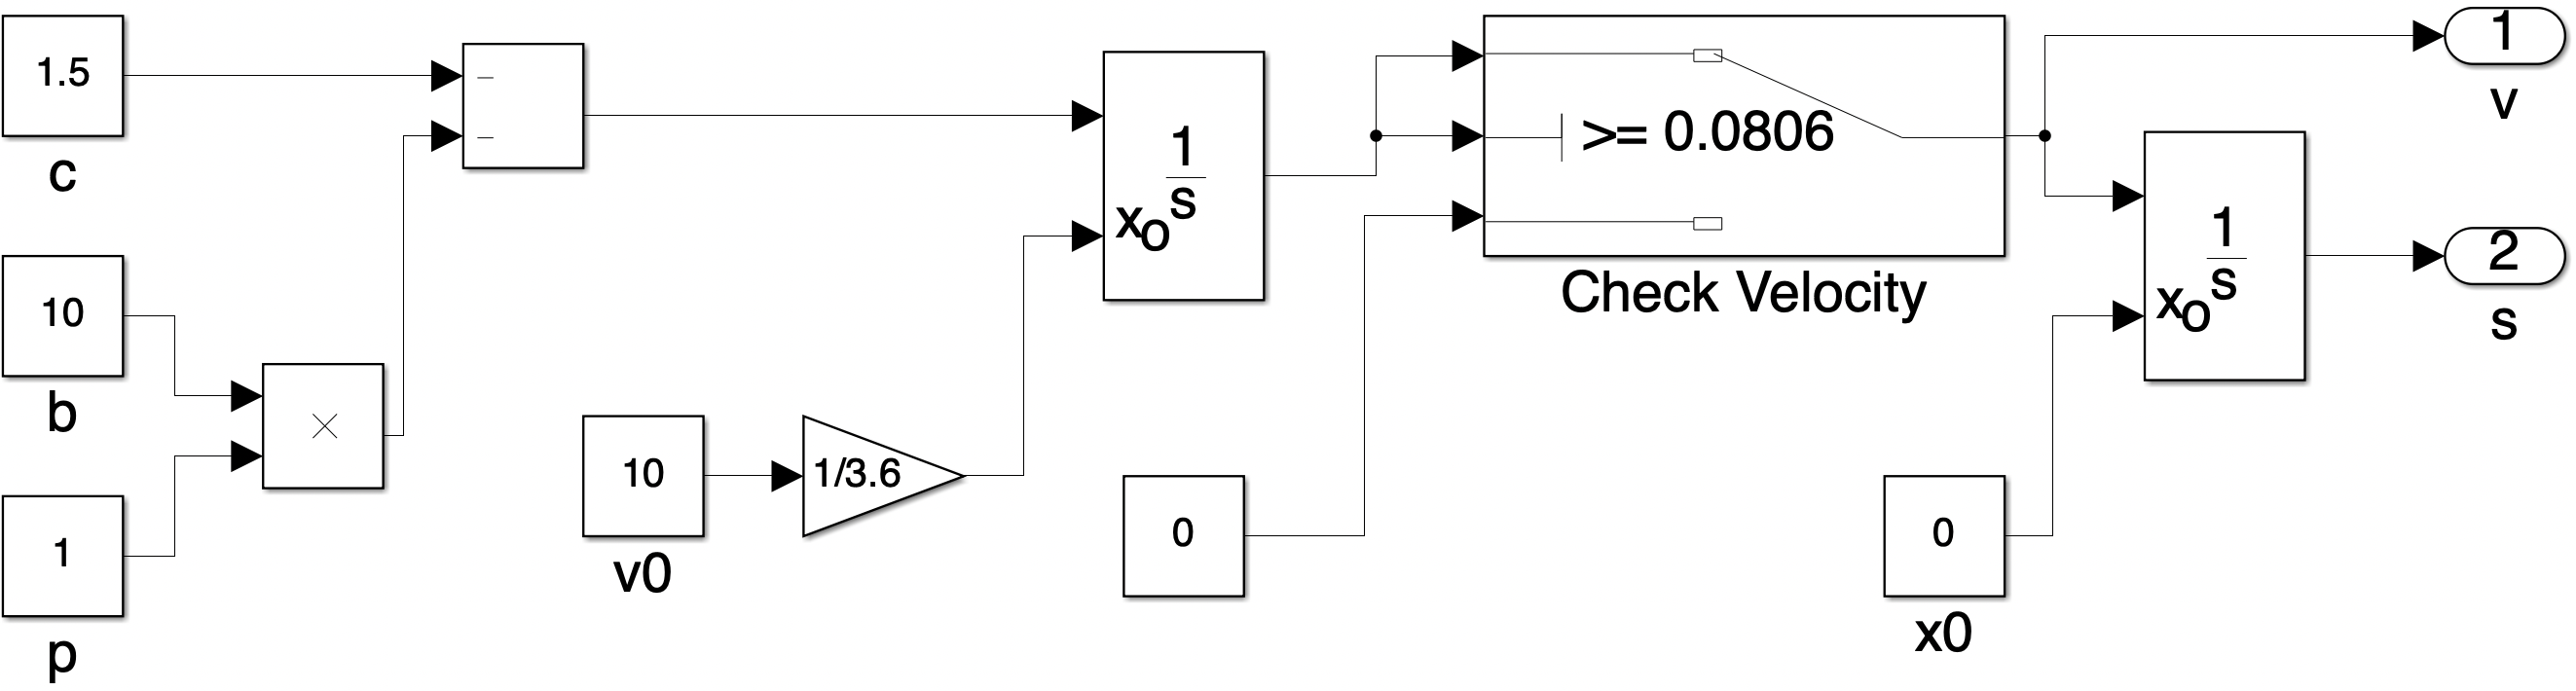
\includegraphics[width=1\textwidth]{images/D2_sim.png}
\caption{Simulink Modell der Differenzialgleichungen}
\label{fig:ConceptArchitectureOverview}
\end{figure}

\chapter{D3: Analysis of human velocity profile}\label{cha:D3}

In this section the provided human velocity profile is analysed in order to find a pattern that shows how a human is breaking a car. This pattern will be used in the following sections and will be adapted to the braking function of the ParkAssist. The analysis is divided into four steps.

\textbf{1. Import the measurement data} \\ The measurement data is imported in Matlab.

\begin{lstlisting}[basicstyle=\scriptsize	,caption= Import measurement data in Matlab,label= lst:D3Import]
%import velocity data
velocity_data = importdata('MeasuredVelocities.txt');
\end{lstlisting}

\textbf{2. Data preparation} \\ Before analysing the data it is necessary to preprocess it. First the four velocities of each wheel are extracted from the measurement data and a mean velocity is calculated (see line 1,2). 

\begin{equation}
	v_{car} = (v_{w1} +v_{w2} + v_{w3} +v_{w4})*4
\end{equation}


The mean velocity is converted to [m/s] for further calculations. For analysing the braking behaviour the acceleration is calculated. This can be done by differentiating the velocity (see line 11). As can be seen in Figure REF in the upper plot the calculated acceleration is ?? as cause of minor variations in the velocity. Due to the ?? it would be hard to analyse the braking behaviour. Therefore, we used a moving average filter to smoothen the data (line 8). A moving average filter is calculating a mean value of neighbourhood elements within a sliding window of a predefined size. Applying a moving average filter results in a smoother graph as can bee seen in the lower plot in Figure REF.

\begin{lstlisting}[basicstyle=\scriptsize	,caption= Preprocessing measurement data,label= lst:D3Preprocess]
%compute mean velocity of all 4 wheels
velocity_per_wheel = velocity_data(:,2:5);
mean_velocity = mean(velocity_per_wheel,2);
mean_velocity = mean_velocity/3.6;      %convert velocity from km/h to m/s
raw_mean_velocity = mean_velocity;      %for demonstration purposes

%apply moving average filter to smoothen the data
mean_velocity = movmean(mean_velocity, 200); 

%differentiate velocity to get acceleration
acceleration = diff(mean_velocity);
raw_acceleration = diff(raw_mean_velocity);     %for demonstration purposes
\end{lstlisting}

\textbf{3. Extracting negative acceleration} \\ As the goal is to analyse the braking behaviour only the negative acceleration is relevant and is thus being extracted from the overall acceleration (line 5). Also, all velocities that are based on a positive acceleration are not considered anymore (line 6). We decided to set those values to \ac{NaN} because this way we are still able to plot the velocity and the acceleration over time without cut-outs. The result can be seen in plot REF.

\begin{lstlisting}[basicstyle=\scriptsize	,caption= Extracting negative acceleration,label= lst:D3Extract]
%search for negative acceleration and set positive acceleration to NaN
%set all velocities that have a positive acceleration to NaN
neg_acceleration = acceleration;
decreasing_velocity = mean_velocity;
neg_acceleration(neg_acceleration>0) = nan;
decreasing_velocity(isnan(neg_acceleration)) = nan;
\end{lstlisting}

\textbf{4. Separating breaking sequences} \\ For improved visualisation the individual breaking sequences that can be seen in plot REF are stored separately. One breaking sequence consists of multiple consequent velocities. This means that the breaking sequences can be separated by searching for a gap in the velocities. Therefore, the indices of all velocities that are set not \ac{NaN} are extracted (line 2) and differentiated (line 3). Considered the differentiation, every differentiation that is greater than 1 marks a gap between velocities because indices of one braking sequence are consequent (differentiation equals 1). Furthermore, small breaking sequences are not considered because they are most likely not relevant for recognizing a breaking pattern (line 13). Two individual breaking sequences can be seen in plot REF and plot REF.

\begin{lstlisting}[basicstyle=\scriptsize	,caption= Separating breaking sequences,label= lst:D3Seperat]
%find individual breaking sequences
notNaN_velocity = find(~isnan(decreasing_velocity));   % find index of every velocity that is not NaN -> one breaking sequence has consequent time steps -> one breaking sequence has consequent indices
diff_notNaN_velocity = diff(notNaN_velocity);          % differentiate indices -> if indices are not consequent (unequal 1), a new breaking sequence has begun
n = 1;                                                 % set start values
start = 1;

%seperate breaking sequences with previous findings
for i=1:length(diff_notNaN_velocity)
    %for every index check if indices are consequent -> equals 1
    if diff_notNaN_velocity(i) > 1
        %if not check if a breaking sequence consists of min 500 time
        %steps, this way small breaking sequences are sorted out
        if (i-start) > 500
            %add breaking sequence to section
            %i is end of sequence
            section{n} = notNaN_velocity(start:i);
            %start for new sequence is end of old sequence + 1
            start = i+1;
            %increment n
            n = n+1;
        else
            %if breaking sequence is to small, set start for new sequence
            %to end of old sequence + 1 anyway
            start = i+1;
        end
    end
end
\end{lstlisting}

\subsubsection{Result}
Considering Figures REF, REF and REF, it can be seen that the acceleration is approximately in the shape of a parable with the minimal turning point at XX. For further implementation of the ParkAssist, we will start the breaking process with an acceleration and increase it until we reach approximately REF and will then decrease it.

%entschieden Durchschnitt der vier Radgeschwindigkeiten zu nehmen (vllt. vor nachteile)
%und so auf die Geschwindigkeit des Autos näherungsweise zu bestimmen
%
%todo hier plot von gesamtgeschwindigkeit
%
%idee: verzögerungsphasen extrahieren um so auf "menschliche" negative beschleunigung zu schließen
%problem: verrauschte messdaten -> dadurch ständiger wehcsel positive negative beschleunigung
%
%lösung: moving average filter zum glätten der messwerte
%dann extrahieren der negativen beschleunigungen

\chapter{D4*: Consideration of uneven parking spaces}\label{cha:D4}
-diagram

-forces need to be considered (hangabtriebskraft)

-negative slope would increase stopping time and position

-positive slope would make stopping time shorter

-negative slope critical since collision could occur

-therefore brake power would have to be increased or decreased

-physical borders need to be considered

-also when the car is stopped it should not start to roll forwards or backwards.
On a plain surface, the brake can be released, after the car is stopped.
A brake assist on a positive or negative slope would need to keep holding the brake or engaging the handbrake.

In the model without a minimum velocity, the velocity would become negative on braking instead of the car coming to a full stop.

\chapter{D5: Discussion of inaccuracies in velocity measurement}\label{cha:D5}
-inaccuracy of velocity +- 0.1 km/h
-also minimal velocity is 0.29 km/h which is not realistic, because velocity does not drop from 0.29 km/h to zero
-in human velocity profile 4 tire velocities recorded
-mean used to compute car velocity
-because of inaccuracy in velocity computed acceleration also has inaccuracy
-car driving around corner
validate findings by numbers from simulation

\chapter{D6: Implementation of pulse signal in Simulink}\label{cha:D6}

\chapter{D7: Transfer of Simulink model to ASCET}\label{cha:D7}

\chapter{D8: Implementation of pule signal in ASCET}\label{cha:D8}

\chapter{D9: Implementation of unit tests for ASCET model parts}\label{cha:D9}
-modular design for unit tests
\chapter{D10: Development and implementation of a system test environment for ASCET simulation}\label{cha:D10}

\chapter{D11*: Plausibility check comparing measured velocities and distances}\label{cha:D11}
-statistically independent ultrasonic distance and velocity
-if distance to next object for ultrasonic sensor is known

-al
\chapter{D13*: Impact of inaccuracies}\label{cha:D13}
-ultrasonic measurement: what if object is round?
-
\chapter{D14*: Reflection}\label{cha:D14}
-only 2 meter stop considered
-model not realistic